\documentclass[12pt,a4paper]{article}
\usepackage[utf8]{inputenc}
\usepackage{amsmath}
\usepackage{amsfonts}
\usepackage{amssymb}
\usepackage{graphicx}
\usepackage{booktabs}
\usepackage{natbib}
\usepackage{dcolumn}
\usepackage{setspace}
\usepackage{array}
\usepackage{pdflscape} %allows for rotating pages with wide tables
\newcolumntype{P}[1]{>{\raggedright\arraybackslash}p{#1}}
%\usepackage{tabulary}
\usepackage[T1]{fontenc}
\usepackage{lmodern}
\usepackage{multirow}
\usepackage{multicol}
\usepackage{todonotes}

\usepackage{mathptmx} %times font
%\usepackage{tgpagella} %palatino font
\usepackage[protrusion=true,expansion=true]{microtype}
\usepackage[top=1in, bottom=1in, left=1in, right=1in]{geometry}
\usepackage[hidelinks]{hyperref}
\usepackage{color,soul} %highlighting
\usepackage[size=footnotesize]{caption}
\captionsetup[figure]{labelfont=bf}
\captionsetup[table]{labelfont=bf}

%\usepackage{endnotes}
%\usepackage[heads,nolists,tablesfirst]{endfloat} %places tables and figures at the end
%

%%making use of footnotesize in all tables
\usepackage{floatrow}
\DeclareFloatFont{tiny}{\footnotesize}% "scriptsize" is defined by floatrow, "tiny" not
\floatsetup[table]{font=footnotesize}

%putting caption on top
\usepackage{float}
\floatstyle{plaintop}
\restylefloat{table}

\usepackage{epstopdf}

\usepackage{etoc}

\title{\textbf{The Conditional Impact of Local Economic Conditions on Incumbent Support}}
%\title{\textbf{Housing Bubbles and \\Support for Incumbents}}


\author{Martin Vinæs Larsen\thanks{Corresponding author. \href{mailto:mvl@ifs.ku.dk}{\texttt{mvl@ifs.ku.dk}}. } \qquad Frederik Hjorth \qquad Peter Thisted  Dinesen \\Department of Political Science \\ University of Copenhagen \and Kim Mannemar  Sønderskov  \\Department of Political Science \\ Aarhus University   }

%,  }  }


\begin{document}
	
	\maketitle
	
	\begin{center}
		\textsc{Presented at the International Conference of Europeanists \\
			July 12-14, University of Glasgow, UK }
		%\\[1em]
		%	please only quote or cite with permission}
	\end{center}
	
	\begin{abstract} \noindent The state of the economy, whether one’s own or that of larger social aggregates, has long been considered among the most important predictors of support for incumbent politicians. Recent studies of economic voting have focused on the role of the local economy, but with inconclusive results. We propose that the impact of the local economy is conditional on which aspects are experientially salient to voters. We provide evidence for this proposition by focusing on the influence of local housing markets on support for the incumbent government. Linking uniquely detailed and comprehensive data on housing sales from Danish public registries to both precinct-level election returns and a two-wave individual-level panel survey, we find that when individuals interact with the housing market, their support for the incumbent government is more responsive to changes in local housing prices. The study thus provides a framework for understanding when citizens respond politically to local economic conditions.
		
	\end{abstract}
	
	%\begin{keyword}
	%\doublespacing
	%%x \sep y
	%\end{keyword}
	
	%\end{frontmatter}
	
	\newpage
	
	\onehalfspacing
	%\doublespacing
	
	\section{Introduction}
	
	\noindent Retrospective evaluations of the state of the economy play at least some role in voters' minds when standing at the ballot box. Voter behavior scholars tend to view retrospective voting as an effective shorthand for evaluating the performance of incumbent politicians and punish and reward them accordingly \citep{ashworth2012electoral,healy2013retrospective}. Yet, the specific aspects of the economy on which retrospective voting is based remain debated. 
	
	Recently, the economic voting literature has turned its attention to the role of local economic conditions. \hl{vinaes, skriv lidt om andy hall o.a. her}
	
%	In this paper, we focus on what we believe to be an understudied economic influence: local housing markets.
	
	In parallel with this attention to the role of local economic conditions in economic conditions, the study of effects of local contexts has enjoyed a resurgence in the political behavior literature. Recent studies of the influence of local contexts have emphasized the role of direct exposure at the neighborhood level as the crucial mechanism underpinning context effects. This theoretical emphasis highlights the importance of salient local events as a precondition for influence of local contexts on political behavior. However, the study of local economic conditions has yet to incorporate this development \citep[though see][]{bisgaard2016reconsidering}.
	
	In this paper, we join these two parallel but largely separate literatures, using insights from the contexts effects literature to provide a framework for understanding when local economic conditions matter for incumbent evaluations. In addition to explaining theoretically why local economic conditions may only sometimes factor into vote choice, it helps resolve the tension between positive and null findings in the existing literature.
	
	We test the observable implications of our framework by examining the relationship between changes in local housing markets and incumbent government support in Denmark, using uniquely detailed and comprehensive data on housing sales. We do this using two complementary empirical approaches. First, we link detailed registry data on local housing prices to election results at the precinct level across four national elections, allowing us to study whether within-district differences in property values are related to support for parties in government. Second, to test the hypothesized causal mechanism that voters make inferences about government based on the state of their local housing market, we zoom in on individual voters' local contexts. Specifically, we link a two-period panel survey to precise measures of how individuals' neighborhoods -- measured at very low levels of aggregation -- were affected by changes in house prices.
	
	We find the hypothesized positive relationship between local housing prices and support for governing parties at both the precinct-level and in the individual-level data. Specifically, a 50 pct. year-on-year increase in local housing prices, equivalent to the sharpest price increases during the housing boom, is associated with a 3 to 5 percentage points increase in the support for governing parties. We find no evidence that housing prices affect the respondents’ ideological orientation, and no evidence that the effect of housing prices on incumbent support depends on whether you own your own home. Furthermore, we show that the effect of housing prices is more pronounced among individuals who are more likely to be attuned to the state of their local housing market -- where local housing market activity is high, and among individuals who have recently or soon will be relocating. Taken together, these analyses suggest that voters do not respond to changes in local housing prices because it changes their preferences for specific policy interventions or their own economic situation, but because of what the local housing market tells them about incumbents' performance.
	
	\section{When local economic conditions affect incumbent support}
	
	The extant economic voting literature has primarily investigated whether voters are responsive to local economic conditions in one of two ways. One set of studies has examined the extent to which voters draw inferences about national economic conditions from local economic conditions \citep{books1999contextual,reeves2012ecologies,anderson2011local,ansolabehere2014mecro}, while another strand of studies have examined the extent to which voters draw inferences about whether to support incumbent politicians  \citep{hansford2015reevaluating,eisenberg2004economic,kim2003spatial,healy2014presidential, hall2017economic,elinder2010local,auberger2005influence}. Studies from both strands of the literature yield inconsistent results finding either small or no effects of local economic conditions on a given outcome.   
	
	Our study distinguishes itself from these previous efforts by highlighting the multi-faceted nature of local economic conditions. The average citizen learns about economic conditions through exposure to a multitude of signals from different economic realms. Though she may learn about national economic aggregates through media consumption, a substantial part of this exposure to economic signals will inevitably come from local informational sources. This may include casual observation of changing supermarket prices, shuttered stores, or job postings. She may also learn about local economic conditions from direct, personal involvement with the local economy through job searching or buying or selling a home. Each of these interactions involves exposure to a particular aspect of the local economy.
	
	The notion that citizens learn about national-level conditions through particular aspects of local economic conditions has a long pedigree in studies of public opinion and voter behavior. Lippmann \citeyearpar[][p. 79]{lippmann1946public} observed that ``we see at best only a phase and an aspect’’ of public events. Discussing learning about economic conditions specifically, Popkin \citeyearpar[][p. 24]{popkin1994reasoning} notes that ``[p]olitical information is acquired while making individual economic decisions and navigating daily life: shoppers learn about inflation of retail prices; home buyers find out the trends in mortgage-loan interest rates; owners of stock follow the Dow-Jones averages (...)’’ \cite[see also][p. 5]{fiorina1981retrospective}. However, even while acknowledging this point, scholars have refrained from theorizing when particular aspects affect citizens’ evaluations of incumbents. 
		
	 We focus on a particular aspect of the local economy, namely housing, for several reasons. First, housing markets saw a global boom followed by a bust in the period around the great recession with severe economic implications for well-being of both individual households and the overall state of the economy. Second, governments influenced the severity of the market crash to a considerable extent through housing and monetary policy, which in turn makes it likely that voters attribute responsibility to them. Third, housing markets are not a monolithic national phenomenon, but vary substantially across geographical contexts, thereby providing voters with highly visible local information by which to assess incumbents. 

	As our first hypothesis, we expect citizens to treat rely on information from local housing markets when assessing the performance of incumbents: 

	\newcommand{\hone}{the local economic conditions hypothesis\ }

	\begin{quote}
		\textit{H1 (Local economic conditions hypothesis): When local house prices rise, individuals are more likely to support the incumbent government.}
	\end{quote}
	
	We argue that in the process of a citizen interacting with a particular aspect of the local economy, that aspect becomes cognitively salient. When she evaluates the incumbent government’s economic performance in the context of vote choice, aspects with which she has interacted more recently are more likely to factor in as “top-of-mind” considerations \citep{zaller1992nature}. The concept of priming in the political psychology literature provides an instructive parallel. Just as media emphasis on particular political issues in the context of a campaign can cause those issues to carry more weight in a citizen’s evaluation of the incumbent, interaction with a particular aspect of the local economy can cause that aspect to carry more weight in her assessment of the state of the local economy in general. In that sense, our argument applies the logic of priming to citizens’ interactions with and evaluations of local economic conditions. 
	
	This leads to out second hypothesis, namely that the association posited in H1 is stronger where local economic activity primes housing market information:
	
	\newcommand{\htwo}{the contextual priming hypothesis\ }
	
	\begin{quote}
	\textit{H2 (Contextual priming hypothesis): The association between changes in local house prices and support for the incumbent government is stronger in more active local housing markets.}
	\end{quote}
	
	This conditional theory of how local economic conditions matter for voters might help explain why previous studies have found inconsistent results. If the impact of local economic conditions depends on which aspects of the local economy citizens interact with, then we should expect the effect of local economic conditions to be moderated by what kind of local economic conditions the study focuses on and by the relation that the electorate has to this part of the economy.
	
	In addition to the literature on the impact of local economic conditions referenced above, our study ties into several neighboring literatures. First, a recently emerged strand of research in political economy highlighting the influence of home ownership -- in itself or as part of a portfolio of economic assets -- on redistribution and social policy preference as well as voting \citep{ansell2014political,nadeau2010patrimonial,stubager2013reaching}. Second, our studies ties into a growing literature on `context effects' exploring the various ways in which political behavior and conditions is shaped by local contexts \hl{(string cite needed here)}. 
	
	\section{Empirical setting}
	
	We study the effect of changes in local housing prices on support for the incumbent government in Denmark in the years surrounding the onset of the Great Recession. The precinct-level data (cf. Section \ref{precinctlevel}) covers the election years of 2005, 2007, 2011, and 2015, whereas the individual-level data (cf. Section \ref{individuallevel}) covers panel survey responses from 2004, 2008, and 2011. Denmark is a particularly useful setting for studying the hypothesized during this period of time due to large temporal variations in housing prices. The boom and bust of the Danish real-estate market before and during the great recession was very dramatic, even by international standards. Figure \ref{hpd} shows the trajectory of Denmark's housing bubble compared with other prominent international cases.
	
	
	
	\begin{figure}[htbp!]
		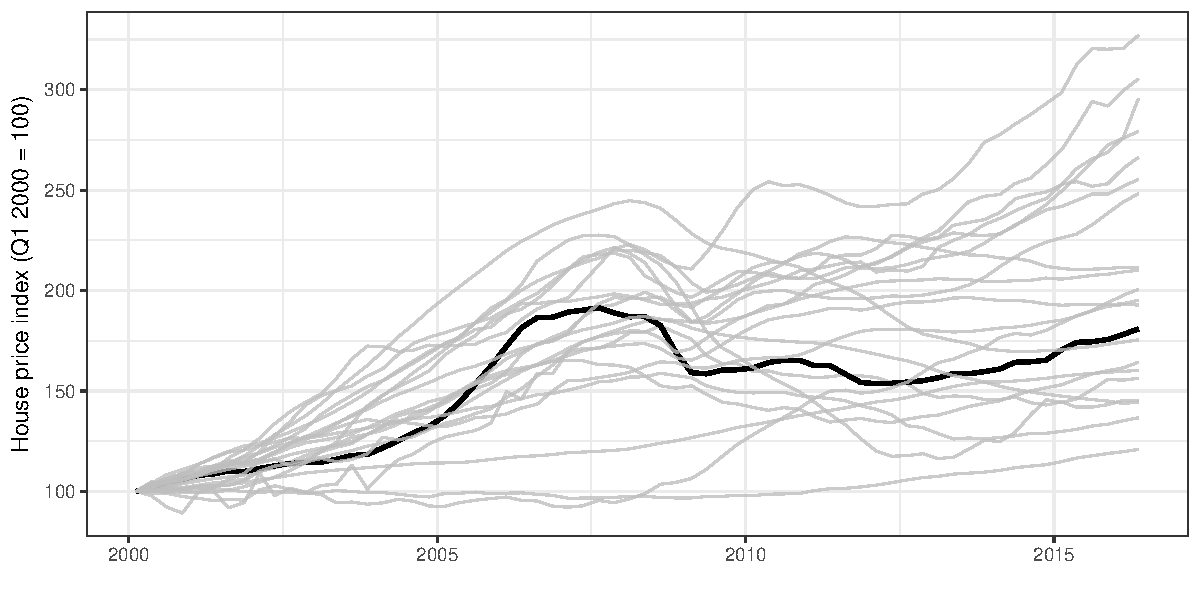
\includegraphics[width=0.9\textwidth]{../figures/timeplot}
		\centering
		\caption{Trends in real house prices in Denmark (black line), Spain, the UK, and the US (dark gray lines) and selected other countries (light gray lines), 2000-2016 (2000 level = 100). Based on the International House Price Database maintained by the Dallas Fed. The authors acknowledge use of the dataset described in Mack and Martinez-Garcia (2011).}\label{hpd}
	\end{figure}
	
	As shown in Figure \ref{hpd}, although many economies experienced large increases in real house prices, Denmark's housing bubble was exceptionally volatile, characterized by a late, rapid increase quickly succeeded by a crash. The bulk of Denmark's housing boom and bust occurred in just four years, from 2005 to 2009. In contrast, the housing bubble in the United States (highlighted in Figure \ref{hpd}), although far bigger in absolute terms, was relatively protracted in comparison. Consequently, local housing markets in Denmark saw year-to-year changes in housing prices that were, even by the standards of a globally economically volatile period, unusually large. This provides us with ample variation in the independent variable of interest.
	
	
	Although the policies exacerbating the housing bubble were implemented by the conservative government, which held office from 2001 to 2011, our argument does not cover only evaluations of the conservative government. If that were the case, evaluations of the government would be observationally indistinguishable from voters becoming more ideologically conservative, a plausible consequence of increases in housing wealth \citep{ ansell2014political}. Below, we distinguish between such an ideological effect of increases in housing prices and a typical non-ideological economic voting effect by investigating whether the size of our effect estimates depend on the ideology of the incumbent government. 
	
	%In Section \ref{inference}, we exploit the change in incumbency in 2011-2015 to show that housing price changes affect support for the incumbent government per se, not merely support for a conservative government.
	
	%Turning to the political context, the government in the entire period we investigate (2005-2015) consisted of two different parties. From 2001 to 2011 the Liberal party was in government along with the Conservative party, and from 2011 till 2015 the Social Democratic party and the Liberal party was in power.\footnote{An additional party, the Socialist party, was in government from 2011 to 2013, however, since this party left government before the election, it is excluded when looking at electoral support for the governing party. To get data on electoral support at the previous election, we also use some data from the 2001 election in which the Social Democratic party and the Liberal party was in power.} This change in party incumbency is useful, since it allows us to distinguish effects on incumbent government support from effects on macropartisanship.
	
	%Housing markets saw a boom followed by a bust in the period around the great recession. This had severe economic implications for wellbeing of both individual households’ and the overall state of the economy \citep{dam2011housing,ansell2014political}. Pairing the economic importance of the housing market with the fact that government regulations (or lack thereof) to a considerable extent influenced the severity of the market crash makes housing markets a particularly useful mean for voters to evaluate the incumbent government by. Furthermore, housing markets are not a monolithic national phenomenon, but vary substantially across geographical contexts, thereby providing voters with relevant local information by which to assess incumbents.
	
	%The second reason we focus on Denmark, is that it is possible to obtain precise and comprehensive data on housing price changes, voting returns, and socio-economic controls at a very small geographic level. Existing approaches typically examine housing price returns at high levels of aggregation corresponding to either counties or entire states. In contrast, we observe housing price changes at the zip code level and voting returns and socio-economic controls at the precinct (i.e., polling place) level. This allows for much more precise measurements of the variables of interest and accordingly less attenuation of observed associations. We elaborate on the specifics of the data in the next section.
	
	\section{Research design}\label{resdesign}
	
	Methodologically, we contribute to the existing literature by exploiting uniquely detailed and comprehensive data on housing market transactions available in Danish public registries. Specifically, we can link highly detailed register data on local housing prices to both precinct-level panel data on national election outcomes as well as individual-level panel survey data. These data ameliorate three methodological challenges confronting the broader class of studies scrutinizing local influences on political attitudes and behavior.
	
	First, we rely on uniquely precise and highly local measures of house prices drawn from public registries. This enables us to address the common problem of confounding local contexts with local media markets -- a very different mechanism -- which, due to data limitations, often arises in studies focusing on local economic conditions in more aggregated geographical contexts \citep[][]{bisgaard2016reconsidering}.  
	
	Second, and related to the previous point, measures of local economic conditions are often based on samples which, while large enough to precisely estimate national economic conditions, typically suffer from insufficient precision when estimating conditions at lower geographical levels \citep[][]{healy2014presidential}. The availability of full-population data allows us to estimate local house prices with high precision.
	
	Third, the panel structure of our data enables us to rule out time-invariant structural differences between local contexts as explanations of any observed relationship between local house prices and support for incumbents by using only within-precinct/individual variation in local housing prices by means of fixed effects. This is particularly important given the strong urban-rural gradient in local economic conditions, which would very likely confound any observed cross-sectional relationship with support for the sitting government.
	
	While some previous studies do address some of these methodological challenges, our study is, to the best of our knowledge, the first to address all of these shortcomings at once. In the remainder of this section, we present in more detail the two data sources we use two test our hypotheses, a precinct-level and an individual-level data set.
	
	\subsection{Precinct-level data}\label{precinctlevel}
	We begin our exploration of the relationship between the state of local housing markets and incumbent support by looking at precinct-level election returns in Danish Parliamentary elections between 2005 and 2015. In particular, we match electoral support for parties in government in these precincts with change in the price of all house sales sold in and around the precincts, examining the extent to which local housing prices and local electoral support for government parties go hand in hand.
	

	The key dependent variable in this analysis is \textit{percent of votes cast for government parties} in each voting precinct. Each voting precinct corresponds to a single polling place, which is the smallest unit at which voting returns can be observed in Danish elections. We measure this for all precincts in four elections:  2005, 2007, 2011 and 2015. There are roughly 1,400 precincts, each precinct consisting of about 3,000 eligible voters on average and covering an average area of 30 square kilometers. A number of precincts are redistricted between each election. This is problematic, as we want to use the precincts as part of a panel data set. There are two ways to deal with this. We can drop precincts as their geographical boundaries get altered. This would mean dropping roughly 15 pct. of the data on the dependent variable. The other option is to fix the precincts geographical boundaries at one reference election (i.e. 2015), and then recalculate vote returns in any changed precincts, so they match up with precincts in the reference election. Since there are a lot of minor changes in geographical boundaries from election to election, and only few major changes, we opt for the latter, which allows us to keep these slightly altered districts in the analysis.\footnote{For details of how returns from the redistricted precincts are calculated, see Søren Risbjerg Thomsen's research note at \texttt{\href{http://bit.ly/205OlPi}{bit.ly/205OlPi}}.  We use 2015 as the reference election.}
	
	The key independent variable is \textit{change in local housing prices}. We obtain housing price data from The Danish Mortgage Banks' Federation (\textit{Realkreditforeningen}), which publishes quarterly data on the average price per square meter of all sales at the zip code level, aggregated from registry data on individual sales.\footnote{Available at \texttt{\href{http://statistik.realkreditforeningen.dk/}{statistik.realkreditforeningen.dk}}.} For each election, we calculate change in housing prices as the percentage change in the price of houses sold in the quarter of the election compared to the same quarter one year before.
	
	Zip codes are a substantively interesting level of aggregation when it comes to the price of housing, as it is the level at which house prices are most often reported in Denmark (cf. the fact they are published by The Danish Mortgage Banks' Federation). However, since the dependent variable is measured at the precinct level, merging these observations is not trivial. Ideally we would extract the zip code of the address of each polling place and link the polling place to housing prices in that zip code. Unfortunately, full addresses are not available for all polling places. Instead, we use a three-stage approach to linking polling places to zip codes. First, we extract the street address and higher-level voting district of each polling place (the full resulting string is of the format `Streetname streetnumber, City, Denmark'). Second, we pass this string to the Google Maps API, which geocodes the string and returns latitude-longitude coordinates.\footnote{Available at \texttt{\href{https://developers.google.com/maps/documentation/geocoding/intro}{developers.google.com/maps/documentation/geocoding/intro}}.} Third and last, we pass these coordinates to the Danish Addresses Web API (DAWA), a public service provided by the Danish Geodata Agency.\footnote{Available at \texttt{\href{http://dawa.aws.dk/}{dawa.aws.dk}}.} The DAWA returns the zip code for each address, allowing us to link polling places to zip codes. %It is important to note that statistically speaking, precincts are therefore nested inside zip codes; we take this into account by clustering the standard errors on the precinct-level in our analysis.
	
	We examine changes in prices rather than price levels. This is in part because the extant economic voting literature, to the extent that it has looked at prices, has also focused on changes (i.e., inflation) rather than levels \citep[cf.][]{kramer1971short}, and in part because it seems likely that changes in housing prices will be more salient for voters than levels. As such, changes in housing prices will translate into either very short or very long turnaround times, as sellers and buyers try to adjust to the new prices, leaving visible traces of these changes in the voters' immediate context -- such as the number of ``for sale'' signs, and the speed at which old neighbors are exchanged for new ones.
	
	In the statistical models, we control for the unemployment rate and median income at the zip-code level in order to isolate local housing markets from other features of the local economy. We also measure the population density ($log(\frac{inhabitants}{km^2})$) of the municipality in which the precinct is located. Like the independent variable, these are all population-based measures calculated from public registries provided by Statistics Denmark.
	
	
	
	\subsection{Individual-level data}\label{individuallevel}
	%In the preceding analysis, we have shown the hypothesized relationship between local housing prices and support for incumbents at the precinct level. While this is quite strong evidence in its own right, replicating this finding using the individual-level data would strengthen its credibility. 
	
	Although our precinct-level data is comprehensive, our hypotheses are at the individual level, and testing individual-level theories with aggregate-level data is fraught with problems of ecological inference. Hence, we include data from a representative sample of Danish citizens in a two-wave panel survey collected between 2002 and 2011. We link the survey respondents to the prices of housing sold in their residential context using the national Danish registers. The registers contain very detailed information about all individuals legally residing in Denmark, including the exact geographical location of their residence, the price of any real estate they sell, and a range of other socio-demographic characteristics \citep{thygesen2011introduction}. This makes it possible to calculate the distance between the individuals in the survey and all other individuals in Denmark and, in turn, the distance to any individuals who are selling their home.
	
	In addition to observing voting behavior at a more theoretically appropriate level, the individual-level data employed also offer a number of features which allow us to probe the hypothesized relationship further. The flexibility and detail of the Danish registers makes it possible to look at multiple levels of aggregation rather than just official levels of aggregation such as zip codes. This makes it possible to reduce concerns related to the modifiable area unit problem (MAUP) in that we can rule out that the findings are tied to a particular way of geographically aggregating housing prices. Furthermore, we can link housing prices to individual-level variables such as attitudes or home ownership, which allow for evaluating plausible alternative explanations. % as well as explore theoretically important individual-level moderators of the housing price effects.
	
	Our independent variable is once again year-over-year changes in housing prices in the residential context of the respondent. We measure the change by comparing the price of housing sold in the quarter prior to the data collection and the price of housing sold in the same quarter a year earlier. Unlike for the precinct-level data, we do not have data on prices per square meter. This makes the individual-level housing price change variable more sensitive to random variation in the types of housing put up for sale in the two time periods we compare. As such, some of the changes from year to year might be due to the fact that larger houses were put up for sale in one year. To take this as well as other structural differences in the type of housing put up for sale into account, we divide the sales price of each unit of housing by its public valuation, before calculating the year-over-year change.\footnote{The Danish government makes a conservative estimate of the price of all housing in Denmark every two years which is used to calculate property taxes. The public evaluation was constant across the time periods we use to estimate housing price changes.}
	
	We estimate the changes in housing prices within each survey respondent's residential context, measuring this context in three different ways. First, and similar to what we did for the precinct-level data, we use the respondents’ zip-code, comparing housing sold within the same zip code a year apart. Second, we look at the prices of the 20 or 40 units of housing sold closest to the respondents own home, comparing the prices of housing sold in the immediate proximity of the respondent to that of housing sold one year earlier. Third, we look at the price of housing sold within a fixed radius of 1000 or 1500 meters of the respondent. These latter ways of defining the respondents’ residential contexts have the benefit of being centered on the respondent, alleviating the problem that the context of a respondent living far from the centroid of one zip-code might be better represented by an adjoining zip-code. Note also that these latter two types of residential context differ in important ways -- whereas the first method takes number of sales as fixed, but varies the geographical dispersion of these sales, the second method holds geographical dispersion fixed, but varies the number of sales. Since it is not obvious which of the three ways of measuring the states local housing market is preferable, we will use them all in the analysis below.\footnote{To do this we use all housing sales registered in the national register EJSA except for those that fall into one or more of the following categories: (1) Sales of part of a house or apartment (10 pct. of all sales). (2) Sales of commercial real estate (9 pct). (3) Sales of apartments or houses valued at more than DKK 10 million (0.2 pct. of all sales) (4) Sales with what `Statistics Denmark' calls an irregular price (i.e. if the sales price is more than three times the valuation or less than forty percent of the valuation, 6 pct. of all sales).}
	
	To get at support for governing parties at the individual level we utilize a two-wave panel survey, constructed by re-interviewing respondents who had participated in the Danish Version of the European Social Survey (ESS); a nationally representative high-quality survey conducted bi-annually in most European countries. The first round of the survey was conducted at three different points in time (round 1, 2 and 4 of the ESS): 2002/3, 2004/5 and 2008/9. In the second round, the full sample of ESS round 1 and 4, and 40 pct. of ESS round 2 (randomly selected), were invited for a re-interview in the winter of 2011-12. In total, 1,745 people -– equivalent to a retention rate of 52 pct. -– were interviewed in both rounds.
	
	The respondents were randomly sampled from the public registry, and therefore the civil registration numbers were retained by the data collection agency. This made it possible to identify the respondents for a second interview and to link the respondents to the national registers. From the survey, we use the following question: ``What party did you vote for at the last parliamentary election?'' Respondents were presented with all the parties which ran in the previous election. For the analyses we create a dummy variable indicating whether the respondent voted for a party in government at the time of the election as the dependent variable.
	
	We also use a number of additional variables in the analysis for statistical control, interaction analyses and placebo tests, which we present as we introduce them in the analysis. 
	
	
	\section{Results}
			
	\subsection{Precinct-level results}
	In Table \ref{predv} we report estimates from a set of linear regression of electoral support for governing parties using changes in local housing prices as the primary independent variable. In all models we use robust standard errors clustered at the precinct-level. In the first column we present a simple linear regression between electoral support and changes in housing prices. In the second column we add year fixed effects, holding trends in incumbent support and rates of housing price changes constant. In column 3 we add precinct fixed effects. In effect, model 3 evaluates if differences in within-precinct changes in housing prices is related to changes in support for the incumbent government. This setup hold averages rates of change constant, and thus effectively eliminate confounding by time-invariant circumstances at the precinct level that may lead to different trajectories in housing prices over time. In column 4 we include the unemployment rate and median income as controls for the trend of the state of the economy in the precinct.
	
	\begin{table}[htbp]\centering
\def\sym#1{\ifmmode^{#1}\else\(^{#1}\)\fi}
\caption{Estimated effects of house prices on electoral support for governing parties.} \label{predv}
\begin{tabular}{l*{4}{c}}
\hline\hline
                    &\multicolumn{1}{c}{(1)}        &\multicolumn{1}{c}{(2)}        &\multicolumn{1}{c}{(3)}        &\multicolumn{1}{c}{(4)}        \\
\hline
$\Delta$ housing price&       0.104\sym{**}&       0.048\sym{**}&       0.053\sym{**}&       0.030\sym{**}\\
                    &     (0.008)        &     (0.007)        &     (0.008)        &     (0.007)        \\
[1em]
Unemployment rate   &                    &                    &                    &      -1.898\sym{**}\\
                    &                    &                    &                    &     (0.221)        \\
[1em]
Log(Median income)  &                    &                    &                    &      -0.891\sym{**}\\
                    &                    &                    &                    &     (0.064)        \\
[1em]
\hline Year FE      &                    &$\checkmark$        &$\checkmark$        &$\checkmark$        \\
[1em]
Precinct FE         &                    &                    &$\checkmark$        &$\checkmark$        \\
\hline
Observations        &        4193        &        4193        &        4193        &        4173        \\
RMSE                &       8.403        &       6.748        &       5.713        &       5.321        \\
\hline\hline
\multicolumn{5}{l}{\footnotesize Standard errors in parentheses}\\
\multicolumn{5}{l}{\footnotesize \sym{*} \(p<0.05\), \sym{**} \(p<0.01\)}\\
\end{tabular}
\end{table}

	
	As can be seen from Table \ref{predv}, there is a statistically significant and positive coefficient attached to changes in housing prices, indicating that a larger fraction of the electorate casts their vote for governing parties in precincts where housing prices are increasing. In the most demanding specification the coefficient is 0.03,  which implies that if the price of housing sold in a precinct's zip-code in the last quarter before the election is twice that of the housing sold in the same quarter the year before, electoral support for  governing parties in this precinct will increase with roughly 3 percentage points.
	
	Unsurprisingly, the effect is larger in the models controlling for fewer variables. The effect size drops from 0.1 to 0.05 when introducing the economic controls, and drops additionally to 0.03 when introducing the time and precinct fixed effects. This highlights the strength of using a difference-in-difference approach and controlling for detailed information about other aspects of the local economy when identifying the effect of local housing prices on incumbent support as this evidently picks up important sources of confounding.
	
	\begin{table}[htbp]\centering
	\def\sym#1{\ifmmode^{#1}\else\(^{#1}\)\fi}
	\caption{Assesing the Robustness of the Precinct-level Evidence} \label{robustness}
	\begin{tabular}{l*{4}{c}}
		\hline\hline
		&\multicolumn{1}{c}{(1)}        &\multicolumn{1}{c}{(2)}        &\multicolumn{1}{c}{(3)}        &\multicolumn{1}{c}{(4)}        \\
\hline
$\Delta$ housing price (2 years)&       0.129\sym{**}&       0.037\sym{**}&       0.022\sym{**}&       0.020\sym{**}\\
&     (0.007)        &     (0.007)        &     (0.007)        &     (0.007)        \\
[1em]
$\Delta$ housing price (FD controls)&       0.104\sym{**}&       0.073\sym{**}&       0.086\sym{**}&       0.058\sym{**}\\
&     (0.008)        &     (0.008)        &     (0.009)        &     (0.008)        \\
[1em]
$\Delta$ housing price (FD DV)&       0.037\sym{**}&       0.034\sym{**}&       0.052\sym{**}&       0.019\sym{**}\\
&     (0.004)        &     (0.004)        &     (0.005)        &     (0.004)        \\
[1em]
$\Delta$ housing price (negative)&      -0.081\sym{***}&      -0.072\sym{***}&      -0.057\sym{**} &      -0.030         \\
&     (0.022)         &     (0.017)         &     (0.019)         &     (0.019)         \\
[1em]
$\Delta$ housing price (positive)&       0.116\sym{***}&       0.045\sym{***}&       0.031\sym{**} &       0.029\sym{*}  \\
&     (0.012)         &     (0.011)         &     (0.011)         &     (0.011)         \\
[1em]
\hline Economic controls  &                    & $\checkmark$                    &$\checkmark$        &$\checkmark$        \\
[1em]
Precinct FE  &                    &                    &$\checkmark$        &$\checkmark$        \\
[1em]
Year FE             &                    &                    &                    &$\checkmark$        \\
\hline\hline
\multicolumn{5}{l}{\footnotesize Standard errors in parentheses}\\
\multicolumn{5}{l}{\footnotesize \sym{*} \(p<0.05\), \sym{**} \(p<0.01\)}\\
\end{tabular}
\end{table}
	
	How robust are these results? In table \ref{robustness} we try to reanalyze the models above in different ways, to get a more complete picture of the statistical evidence for (or against) the importance of local housing markets for incumbent support.
	
	We begin by looking at whether the chosen time period, i.e. year-over-year changes, impinges on out results. To do so we reestimate the models from table \ref{predv} using the change in housing prices over two years rather than just one. The results, reported in the first row in Table 2, are fairly similar using this measure of more long run changes in housing prices, although the estimated effects tend to be smaller than what we found above. This squares with previous work showing that voters are, by and large, myopic when it comes to relating economic indicators to incumbent support \citep{healy2009myopic,healy2014substituting}.
	
	As mentioned above, we use changes in house prices rather than levels. However, in our models we control for the level of income and the level of unemployment. One could imagine, that this means that we fail to capture something important about how the economic status of the precinct is changing, which could in turn confound the effect of changes in housing prices. To examine whether this is the case, we re-estimate the different models using first-differenced (FD) controls. As can be seen in the third row of table \ref{robustness}, this does not alter the main conclusion. In fact, the estimated effects of local housing prices doubles in size in this specification. We also estimated a set of complete change models, using an FD dependent variable as well. The estimates from these models are reported in the fourth row of the table. The estimated effect size of housing prices in the completely differenced model is somewhat smaller than what was identified in table \ref{predv}, but it remains statistically significant in the mode demanding models.
	
	Another concern relates to whether the effect is only present for right wing incumbents. In particular, one might argue that as housing prices in an area increases, the wealth of the voters living in this area also increases, and this might lead to increased support for right wing politicians \cite{ansell2014political}. This problem is especially acute in this context, as the government parties in power from 2001 to 2011 were right wing. To address this issue we re-estimate our models using data from the 2011 and 2015 elections in the fourth row. The fourth and fifth model, which includes precinct fixed effects, are of special interest. The estimates from these models tell us whether voters were more likely to vote for the left-wing incumbent in 2015 than the right wing incumbent in 2011 in precincts where the local housing market was doing better in 2015 than in 2011 (i.e., it is similar to a two period first difference model). The estimates reveal that voters were more likely to vote for a left-wing incumbent when local housing prices were increasing. In fact, the estimated effect size is substantially larger when analyzing this subset of data. This is important because it suggests that the relationship between changes in local housing prices and support for incumbent governments is a more general phenomenon and not confined to right-wing incumbents. By implication, this allow us to rule out that the relationship is driven by the electorate becoming more conservative due to increases in housing wealth.
	
	As a final robustness test, we split the housing price variable in two, creating one variable which measures the size of positive changes, which is zero if there is a negative change, and one variable which measures the size of negative changes, which is zero if there is a positive change. This makes it possible to study the effect of increases and decreases in housing prices separately. We report the result of these analyses in the two last rows of table \ref{robustness}. Interestingly, the effect of negative changes and positive changes do not seem to differ - they are both roughly 0.03. This is important because it shows that voters reward governing politicians when house prices are on the rise, and then punish them when they fall. This may be seen as somewhat surprising, because much previous research have found that voters respond more strongly to negative economic conditions \citep[e.g.][]{bloom1975voter,headrick1991attention,soroka2014negativity}.
	
	Taken together, these analyses suggest that there is a robust, positive effect of local housing prices on support for governing parties.
	
%	\subsubsection{Local economic activity as moderator}
	
	xx 
	
	
	\begin{table}[htbp]\centering
\def\sym#1{\ifmmode^{#1}\else\(^{#1}\)\fi}
\caption{Estimated effects of housing price across number of trades.} \ref{table:econactivity}} \label{prelagiv}
\begin{tabular}{l*{4}{c}}
\hline\hline
                    &\multicolumn{1}{c}{(1)}        &\multicolumn{1}{c}{(2)}        &\multicolumn{1}{c}{(3)}        &\multicolumn{1}{c}{(4)}        \\
\hline
$\Delta$ housing price&      -0.039        &      -0.102\sym{**}&      -0.077\sym{**}&      -0.079\sym{**}\\
                    &     (0.027)        &     (0.021)        &     (0.023)        &     (0.023)        \\
[1em]
$\Delta$ housing price $\times$ logntrades&       0.049\sym{**}&       0.050\sym{**}&       0.038\sym{**}&       0.033\sym{**}\\
                    &     (0.008)        &     (0.007)        &     (0.007)        &     (0.007)        \\
[1em]
Unemployment rate   &                    &                    &                    &      -1.656\sym{**}\\
                    &                    &                    &                    &     (0.217)        \\
[1em]
Log(Median income)  &                    &                    &                    &      -0.856\sym{**}\\
                    &                    &                    &                    &     (0.063)        \\
[1em]
\hline Precinct FE  &                    &                    &$\checkmark$        &$\checkmark$        \\
[1em]
Year FE             &                    &$\checkmark$        &$\checkmark$        &$\checkmark$        \\
\hline
Observations        &        4195        &        4195        &        4195        &        4175        \\
RMSE                &       8.501        &       6.736        &       5.637        &       5.288        \\
\hline\hline
\multicolumn{5}{l}{\footnotesize Standard errors in parentheses}\\
\multicolumn{5}{l}{\footnotesize \sym{*} \(p<0.05\), \sym{**} \(p<0.01\)}\\
\end{tabular}
\end{table}

	
	xx
	
	\begin{figure}[htbp!]
		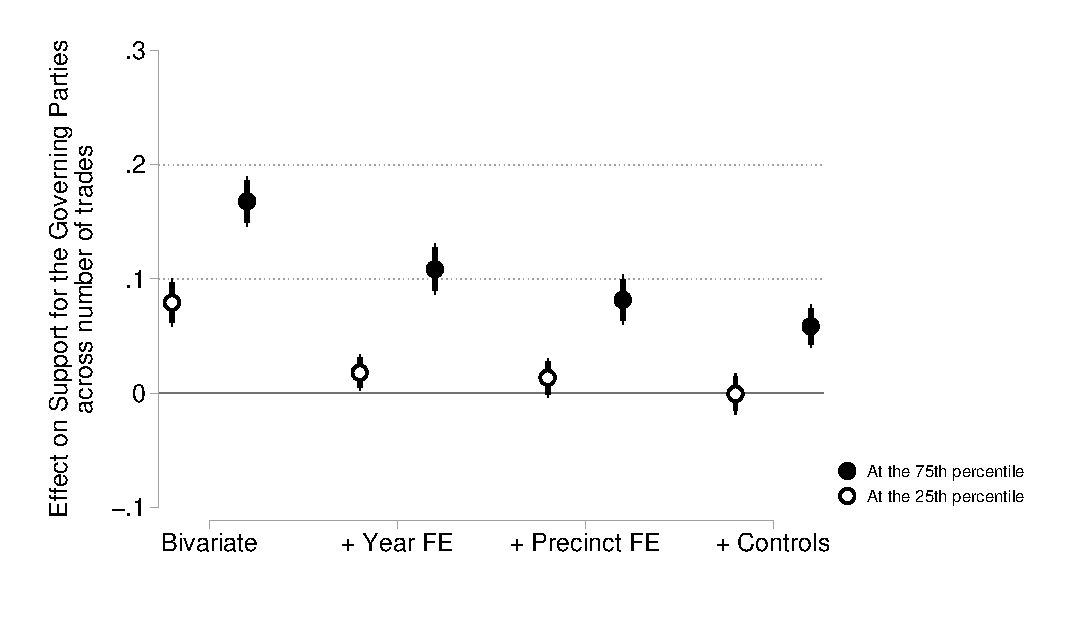
\includegraphics[width=0.9\textwidth]{../figures/localactivity.eps}
		\centering
		\caption{Average marginal effects of Housing Prices across levels of economic activity with 90  and 95 pct. Confidence Intervals.  Average marginal effects derived based on table \ref{econactivity} at the median of the lower and upper tercile.}\label{comparison}
	\end{figure}
	
	
%	\subsubsection{The parallel trends assumption}
	Another potential threat to our results is that that the effect of local housing markets on support for incumbents is simply a reflection of some secular trend predating the housing bubble—i.e., that governing parties already becoming more/less popular in places where housing prices eventually increase/decrease—in. To address this we estimate the same type of models as in table \ref{predv}, using support for the governing party at the last election as the dependent variable (the lagged dependent variable). We plot the estimated effects of housing prices on the lagged dependent variable, as well as on the actual dependent variable, in figure \ref{placebo}. As can be seen from this figure there is an significant effect of housing prices on the lagged dependent variable in the less restrictive models, however, in the final model, the estimated effect of housing prices is 0.005 -- less than a sixth of the estimate in the corresponding model in table \ref{predv} -- and statistically insignificant. This is important, because a key assumption underlying the difference-in-difference design employed here is that prior trends in the dependent variable are uncorrelated with the independent variable (i.e. the parallel trends assumption). This analysis seems to suggest that no such correlation exists.
	
	\begin{figure}[htbp!]
		\includegraphics[width=0.9\textwidth]{../figures/lagdv.eps}
		\centering
		\caption{Effects of Housing Prices on support for governing party at the present election (t) and the last election (t-1) with 90  and 95 pct. Confidence Intervals}\label{placebo}
	\end{figure}
	
	\subsection{Individual-level results}
	In table \ref{inddv} we report estimates from a set of linear probability models (LPM), setting the probability of voting for a party in government as a function of changes in local housing prices. We estimate the models using a linear regression with fixed effects for the respondent, and fixed effect for which of the four different survey rounds the respondent is participating (ESS round one, two, four or the re-interview). All models include controls for the average income and unemployment rate in the respondents’ context, as well as indicators of the respondent's own income and whether someone in the household is unemployed. Like in the precinct-level analyses, this is to differentiate the effect of local housing markets from that of other personal of local economic variables. However, unlike for the precinct level data we can now control for trends in both the individuals personal economy and for the economy of the larger context. In effect, we end up with a difference-in-difference model, which controls for trends in the economic situation. We use robust standard errors, clustered at the individual level.
	
	All models include the same set of variables, but they differ in how the contextual variables are defined. In column one we present a model where housing price change is calculated based on the 20 closest sales (cf. above), and where the other contextual variables -- average income and unemployment rate -- is measured within a 500 meter radius of the respondent. In column two we use the 40 closest sales, but leaves the remaining variables measured as in column one. In column three and four, we define all contextual variables, sales, unemployment rate and average income, as 1000 and 1500 meter radii around the respondent. Finally, in column five, we examine sales at the level of zip codes, but the other contextual variables are calculated based on people within a 1500 meter radii around the respondent.
	
	\begin{table}[htbp]\centering
\def\sym#1{\ifmmode^{#1}\else\(^{#1}\)\fi}
\caption{Linear Regression of Voting for Governing party } \label{inddv}
\begin{tabular}{l*{5}{c}}
\hline\hline
                    &\multicolumn{1}{c}{20 Closest}&\multicolumn{1}{c}{40 Closest}&\multicolumn{1}{c}{1000 metres}&\multicolumn{1}{c}{1500 metres}&\multicolumn{1}{c}{Zip code}\\
\hline
$\Delta$ housing prices&       0.035       &       0.056       &       0.064       &       0.114\sym{*}&       0.063       \\
                    &     (0.036)       &     (0.044)       &     (0.052)       &     (0.051)       &     (0.056)       \\
[1em]
Unemployment rate   &       0.052       &       0.056       &      -0.439       &       0.755       &       0.796\sym{+}\\
                    &     (0.290)       &     (0.289)       &     (0.627)       &     (0.575)       &     (0.422)       \\
[1em]
Average income      &      -0.004       &      -0.004       &      -0.005       &      -0.005       &      -0.006       \\
                    &     (0.003)       &     (0.003)       &     (0.007)       &     (0.007)       &     (0.006)       \\
[1em]
Personal income     &      -0.000       &      -0.000       &      -0.000       &      -0.000       &      -0.000       \\
                    &     (0.000)       &     (0.000)       &     (0.001)       &     (0.001)       &     (0.000)       \\
[1em]
Unnemployed (household)&      -0.032       &      -0.033       &      -0.066       &      -0.048       &      -0.034       \\
                    &     (0.035)       &     (0.035)       &     (0.043)       &     (0.040)       &     (0.036)       \\
[1em]
\hline  Round FE    &         Yes       &         Yes       &         Yes       &         Yes       &         Yes       \\
[1em]
Individual FE            &         Yes       &         Yes       &         Yes       &         Yes       &         Yes       \\
\hline
Observations        &        3479       &        3479       &        2790       &        2992       &        3384       \\
\hline\hline
\multicolumn{6}{l}{\footnotesize Standard errors in parentheses}\\
\multicolumn{6}{l}{\footnotesize \sym{+} \(p<0.1\), \sym{*} \(p<0.05\)}\\
\end{tabular}
\end{table}

	
	The estimated coefficients are positive across the different models, although the size of the coefficient varies somewhat, ranging from 0.04 to 0.11. The effect is only statistically significantly different from zero in one of the five specification -- the one which looks at the 1500 meter context.
	
	While we only observe a statistically significant relationship between changes in house prices and voting for incumbent in one out of five models, and as such should be careful to put too much emphasis on the results, it is important to note that the estimated relationships are actually consistent with what we found in the precinct-level data. To see this figure \ref{comparison} plots the estimated effect of housing prices estimated for the individual-level data in table \ref{inddv}  and for the precinct-level data in table \ref{predv}.
	
	\begin{figure}[htbp!]
		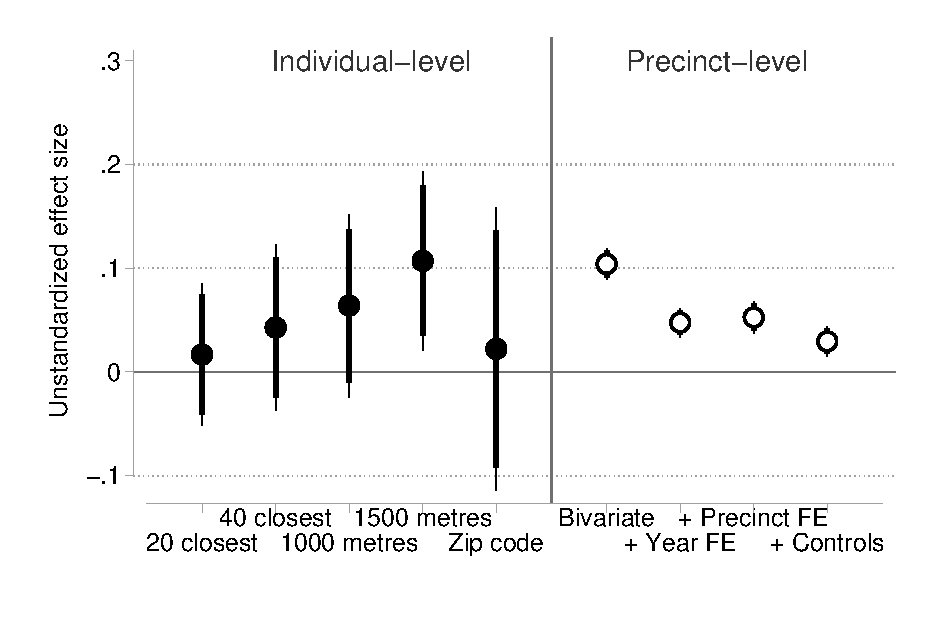
\includegraphics[width=0.9\textwidth]{../figures/comparison.eps}
		\centering
		\caption{Effects of Housing Prices across levels of analysis with 90  and 95 pct. Confidence Intervals}\label{comparison}
	\end{figure}
	
	As is clear from the figure, the effect sizes are pretty similar across levels of analysis - if anything they are larger for the individual level data. This tentatively suggests that that the estimated coefficients do not represent a true null-effect, but rather an imprecisely estimated effect. One plausible reason for this imprecision is measurement error in the dependent variable as voter recall data are known to be erroneously reported (ref.). Furthermore, as we show in the next section, we find statistically significant effect for a sub-group, which can be expected to be especially attuned to hosing prices.
	
%	\subsubsection{Own economic activity as moderator}
	
	%\subsection{Self-interest, Ideology or Inference}\label{inference}
	%
	% As noted previously. \cite{ansell2014political} finds in a recent study that people become more right-wing, in the sense of being less supportive of redistribution, if the price of their home increases. Since there was a Conservative government in office for most of the period we study (2001-2011), this poses the question as to whether our results can be explained by a link between voters ideological position and changes in local housing prices (i.e. that people voted for the conservative government when housing prices increased because they became more conservative).
	%
	%We probed this alternative explanation in the precinct-level analyses, but can investigate it further in the individual-level data. More specifically, we estimate the same models as in table \ref{inddv}, substituting incumbent support for ideological self-placement on a ten point scale going from `Left' to `Right'. For this analysis we rescale the ideology variable to go between zero and one. We plot the estimated effects of changes in housing prices on ideological orientation in figure \ref{ideology}. For comparison, we also plot the effects on incumbent support. As can be seen from the figure there is no discernible effect on ideology, the estimated effects being very close to zero in all models. There is thus little indication that changes in ideology driving our results.
	%
	%
	%\begin{figure}[htbp!]
	%	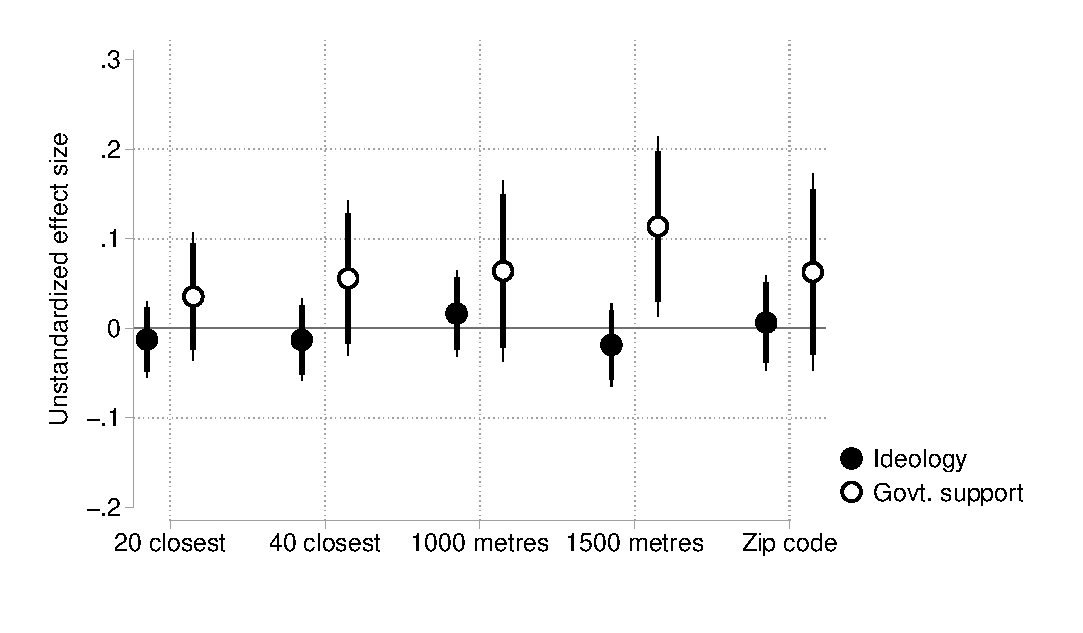
\includegraphics[width=0.9\textwidth]{../figures/ideology.eps}
	%	\centering
	%	\caption{Effects of Housing Prices on Ideological Orientation and Support for Governing Parties with 90  and 95 pct. Confidence Intervals}\label{ideology}
	%\end{figure}
	%
	%A related question is whether voters’ reaction to housing prices are shaped by self-interest. That is, are voters responsive to changes local housing prices because they believe these changes indicate that their own home is worth more. 
	%
	%To examine this we re-estimated the different individual-level models, including an interaction between whether voters owned their own home (i.e. owned or rented), and changes in housing prices. We then derived the estimated marginal effects of changes in housing prices for home owners and others. These marginal effects are plotted in figure \ref{homeown}.
	%
	%The results are a bit mixed with some models showing effects to be slightly larger for home owners, and other models showing no difference. On balance, however, there does not seem to be any systematic evidence for the conjecture that it is only home owners that are affected by changes in housing prices. 
	%
	%\begin{figure}[htbp!]
	%	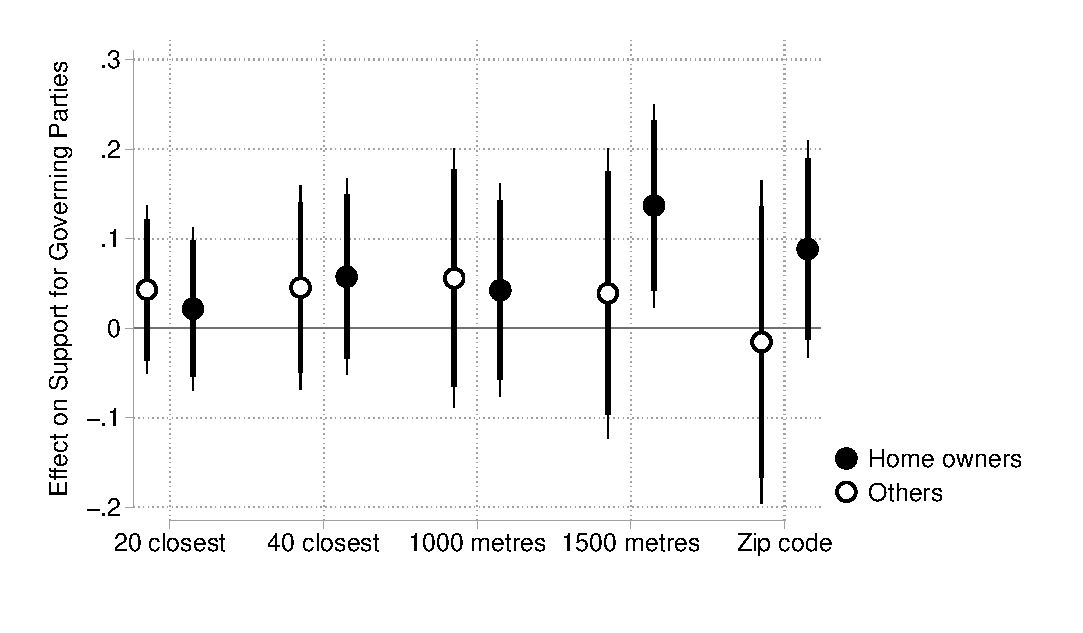
\includegraphics[width=0.9\textwidth]{../figures/homeown.eps}
	%	\centering
	%	\caption{Effects of Housing Prices for those who own their home and those who do not with 90  and 95 pct. Confidence Intervals}\label{homeown}
	%\end{figure}
	
	Why might people who do not own any housing be affected by changes in local housing prices? One reason, which we alluded to in the beginning of the paper, is that local housing markets serve as a signal of the incumbents' competence. As such, even though you do not own your home, you might infer from a booming local housing market, that incumbent politicians are doing a good job keeping your local community economically vibrant.
	
	If voters are in fact using local housing markets as a signal of incumbent quality, we would expect those who are more finely attuned to this signal to be more affected by changes local housing prices.
	
	To test this, we constructed a variable from the national registers, which tries to measure whether the respondent was likely to be attuned to the housing market. In particular, we measure whether the respondent moved within two years before or after being surveyed. To take into account that respondents who moved within one year of being surveyed were probably more attuned than those who moved within two years, we gave respondents a score of one if they moved out the day after or before being surveyed, and then we let the score steadily decline until after two years it was zero (e.g. if you move exactly one year before or after being surveyed you had a score of 0.5). We re-estimate the individual-level models interacting this moving-variable with the housing price change variable.
	
	In figure \ref{move} we derive marginal effects from the different models for those who had not moved within two years (i.e. scores 0) and the effect for those who moved the day before or after answering survey (i.e. scores 1). The estimated effect of housing prices is very large for those respondents who are on the cusp of moving, and, more importantly, is statistically significant in all specifications ($p<.05$ for all models except the zip-code model,$p<.1$ for the zip-code model). The marginal effects for the movers is also significantly larger than the effects for the stayers ($p<0.1$) in four out of the five specifications.
	
	\begin{figure}[htbp!]
		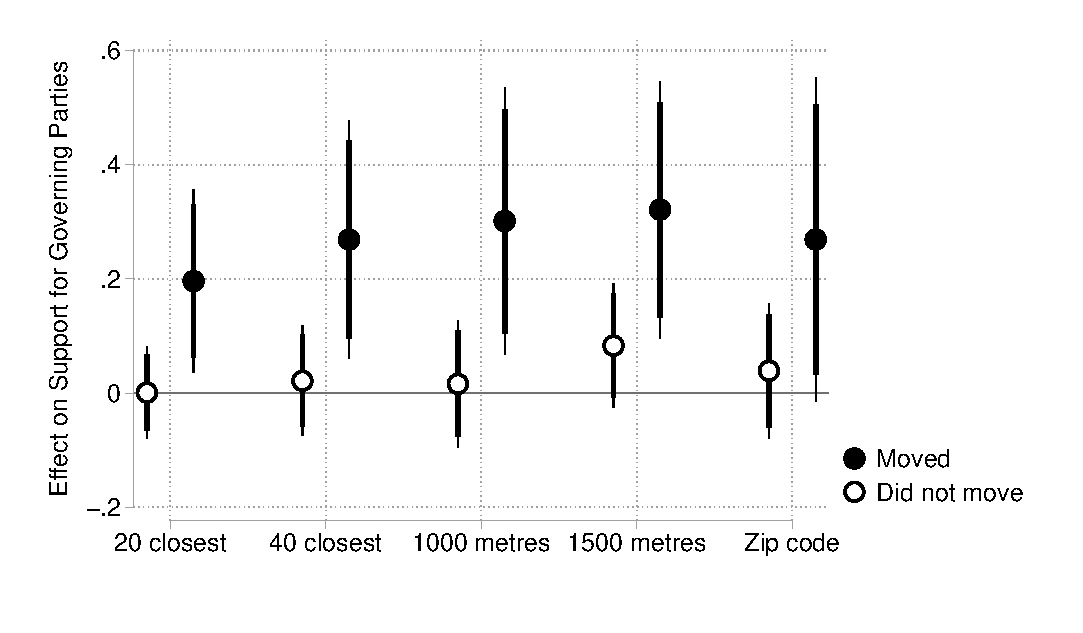
\includegraphics[width=0.9\textwidth]{../figures/moving.eps}
		\centering
		\caption{Effects of Changes in Housing Prices for those who had just or were going to move and those who did not with 90 and 95 pct. Confidence Intervals}\label{move}
	\end{figure}
	
	Taken together, these analyses suggest that the housing price effect is not related to ideology or `simple' self-interest. Instead, to the extent that voters are attuned to local housing markets, changes in local housing prices seems to convey a signal to voters about the incumbent's competence in handling the local economy.
	
	
	
	\section{Conclusion}
	The price of housing tells you something fundamental about the state of the economy in a community. Just like unemployment or local economic growth, housing prices shape the experience and the fate of a community. Therefore housing prices might play an important role in politics. In this article we examined one possible political effect of changes in local housing prices – that on support for incumbents parties. Using precinct-level data on four Danish Parliamentary elections bookended by a dramatic bubble in real-estate prices, we found a positive effect of changes in housing prices on electoral support. Our results suggest that as housing prices increase, so does electoral support for governing parties. Linking a two-wave panel survey of Danish voters to the national Danish registers, we replicated this finding, identifying a comparable effect of housing prices on incumbent support. Analyzing the panel data in more detail, we found that the effect of housing prices was especially pronounced among those who were more likely to be attuned to the local housing market. 
	
	Though the data used in this study is a clear improvement compared to those in earlier studies, it is nonetheless observational. In the absence of fully or quasi-experimental variation in housing prices, we cannot be sure that the estimated effects are not confounded by unobserved heterogeneity. This concern remains even though we apply highly stringent tests to the effect estimate. Hence, a promising avenue for future research is to identify settings with plausibly exogenous variation \citep[cf.]{jerzak2016property}.
	
	What implications do these findings have? First, politicians should care about housing prices and the policies that influence them. If not they risk facing electoral retribution. Further, since voters are sensitive to  local differences in housing prices, politicians cannot simply be attentive to national housing prices, but have to worry about the geographic distribution of any housing booms and busts \citep[cf.][11]{ferejohn1986incumbent}. This aspect, that voters care about local economic conditions, is especially interesting in light of the fact that most studies of the electoral effects of the economy have focused on the national economy or, to a lesser extent, personal economic conditions.
	
	
	
	% LEFTOVERS
	
	%First of all, just like we can learn about political business cycles from studying voter myopia \citep{healy2014substituting,tufte1980political}, or learn about the prevalence of disaster relief vis-à-vis disaster prevention by looking at how voters reward spending on one or the other \citep{healy2009myopic,ashworth2012electoral}, studying how voters react to housing bubbles tells us something about the political antecedents of these bubbles. Specifically, it highlights the incentives reelection-minded politicians face when developing policies which influence the formation of economic bubbles.
	
	%Housing prices tell you something fundamental about the economic situation of  a local community. Just like unemployment or local economic growth, housing prices shape the experience and the fate of a community. Therefore housing prices might play an important role in politics. In this article we wanted to examine one possible political effect of changes in local housing prices -- that on support for governing parties in Denmark. Using precinct-level data on four Danish Parliamentary elections bookended by a dramatic economic bubble in real-estate prices, we found a positive effect of changes in housing prices on electoral support. Our results suggest that as housing prices increase, so does electoral support for governing parties. Does this reflect a causal relationship? While it is notoriously hard to know for sure using observational data, we have shown suggestive evidence that the effect is in fact causal. We have also shown that there is substantial heterogeneity in the effect. Specifically, negative changes seem to have larger effects than positive changes, and changes in areas where prices are more volatile seem to have larger effects than changes in areas, in which prices are less volatile.
	
	%The observed heterogeneities in the effects of housing prices lend themselves easily to conclusions about the motivations of voters punishing or rewarding government parties. Specifically, the stronger observed effect for negative changes over positive ones might lead one to conclude that voters suffer from negativity bias. Conversely, the stronger observed effect in high-volatility areas suggests that voters attempt to parse out the `policy-elasticity' of observed housing price changes.
	
	%Both of these explanations may account for the effects observed here, but caution is warranted when inferring individual-level motivations from aggregate-level effects. Instead, we would argue that the main implications of these findings is not about the rationality of individual voters, but rather the incentives faced by governments. Specifically, the results of this study suggest that even for narrowly office-seeking, myopic governments would not benefit from policies that inflate housing bubbles. Regardless of their motivations, voters systematically react strongly to bubble-like housing price volatility and punish downturns significantly more than they reward upturns. The evidence thus implies that the expected ballot box gains of inflating housing bubbles are negative.
	
	
	
	
	
	
	.
	
	
	
	
	
	\clearpage
	
	\singlespacing
	
	\bibliographystyle{apa}
	\bibliography{library}
	
	\newpage
	
	\appendix
	\section*{Appendix}
	\renewcommand{\thesubsection}{\Alph{subsection}}
	\renewcommand{\thetable}{\Alph{subsection}\arabic{table}}
	
	\localtableofcontents
	
	\subsection{Descriptive statistics}
	\setcounter{table}{0}
	
	Table of descriptive statistics
	
	\newpage
	
	\subsection{Identification strategy}
	
	In this article we want to identify the causal effect of recent changes in precinct level housing prices on electoral support for governing parties. Ideally, we would like to compare support for governing parties in the same district at a specific election across different levels of house-prices. As precincts were only assigned one change in housing prices per election, this is obviously not feasible. Instead, we need to construct a feasible observable counterfactual to a precinct with a specific change in housing prices, which we can use to difference out the effect of housing prices.
	
	One way to do this is to simply compare incumbent support at different levels of housing price changes across elections and within precincts. Here the counterfactual for any given precinct is the incumbent support of an cross-elections average precinct. A key challenge to causal identification in this case is that certain structural features of precincts in which housing prices are likely to increase might make incumbents more popular.
	
	We can begin to deal with this problem by examining the historical precinct-specific levels of incumbent support. As such, instead of simply using an average of all precincts as our counterfactual, we can use the average for the individual precinct. Comparing incumbent support within precincts and across different levels of housing prices. This takes into account that certain precincts might be historically more inclined to support incumbents and have increasing housing prices. However, it does not take into account that when housing prices are relatively high in a district in a particular election, it is also likely to be high in other precincts as well. This is problematic if incumbents do systematically better or worse, in general, when housing prices are doing well.
	
	To address this problem, we can examine levels of incumbents support, not just relative to the precincts history, but also relative to the level of incumbent support across districts. In this case, our counterfactual for any given precinct is the electoral support that governing parties typically obtain in that precinct, plus or minus the overall change in electoral support for governing parties across all precincts. This is a generalized difference-in-difference approach to identifying the effect of housing prices. As such, we look at differences within elections in differences between the individual precincts typical and actual outcome.
	
	The difference-in-differences approach makes it possible to compare with a very reasonable counterfactual situation -- what is the typical incumbent support we could expect in a precinct given the overall popularity of the incumbent. However, since the the governing parties change from election to election, and since the priorities of the same parties might change from election to election, different types of precincts might prefer government parties at  different elections. This poses a challenge to causal identification. As such,  these changes in election and precinct-specific preferences might not be the same across types of precincts which experience increasing and decreasing in housing prices. We cannot completely deal with this problem: As mentioned in the beginning of this section, we have only one piece of information on the assigned housing price change for a precinct at an individual election. However, we can create an even more appropriate counter-factual by taking into account how precincts of a specific type do at specific elections.
	
	First, we can take the precincts economic status into account. That is, how the incumbent scores on the four structural variables mentioned above: income, wealth, employment and benefits. In this case our counterfactual for any precinct will be be the typical incumbent support we would expect a precinct to have given how popular the incumbent is at this specific election in precincts with a similar economic make-up.
	
	Second, we can take the precincts geographical location into account. Specifically, we can look at what municipality,  the smallest local administrative unit in Denmark, the municipality is located in. In this case our counterfactual for any precinct will be be the typical incumbent support we would expect a precinct to have given how popular the incumbent is at this specific election in precincts in the same municipality.
	
	This counter-factual can be expressed using the following linear equation.
	
	\begin{equation}
	y_{it}= \delta houseprices_{it} + \pi_i + year_{it} + \epsilon_{it}
	\end{equation}
	
	Where $y_{it}$ is incumbent support at election $t$ in precinct $i$ and $houseprices_{it}$ is year-over-year changes in housing prices. $\delta$ is the coefficient of interest, as it represents the effect of housing prices on incumbent support.  $\pi_i$ represent precinct fixed-effects and $\epsilon_{it}$ is an error term. $year_{it}$ is a year and precinct specific term, which signifies how much more or less popular, we would expect the incumbent to be in an individual precinct at a specific election, given its geographical location and economic status. It is defined as
	
	\begin{equation}
	year_{it}=\mathbf{X_i\beta_t + Z_i\gamma_t}
	\end{equation}
	
	$ \mathbf{X_i}$ is a vector of the four economic variables and $\mathbf{\beta_t}$ is a vector of coefficients attached to these variables, which specify the relationship between these variables and incumbent popularity at time $t$. $\mathbf{Z_i}$ is a vector of 98 dummy variables indicating which of 98 municipalities the precinct lies within. $\mathbf{\gamma_t}$ is a vector of coefficients attached to these dummy variables, which specify the cross-precinct municipal average of incumbent popularity at time $t$.
	
	As a test of the parallel trends assumption, in Table \ref{prelagdv} we look at whether housing prices can predict changes in support for governing parties in the last period.
	
	
	\begin{table}[htbp]\centering
\def\sym#1{\ifmmode^{#1}\else\(^{#1}\)\fi}
\caption{Estimated effects of house prices on electoral support for governing parties at t-1.} \label{prelagdv}
\begin{tabular}{l*{4}{c}}
\hline\hline
                    &\multicolumn{1}{c}{(1)}        &\multicolumn{1}{c}{(2)}        &\multicolumn{1}{c}{(3)}        &\multicolumn{1}{c}{(4)}        \\
\hline
$\Delta$ housing price (lag DV)&      -0.021\sym{**}&      -0.034\sym{**}&      -0.029\sym{**}&       0.008\sym{**}\\
                    &     (0.007)        &     (0.004)        &     (0.003)        &     (0.003)        \\
[1em]
\hline Precinct FE  &                    &                    &$\checkmark$        &$\checkmark$        \\
[1em]
Year FE             &                    &                    &                    &$\checkmark$        \\
\hline
Observations        &        3099        &        3089        &        3089        &        3089        \\
RMSE                &       4.430        &       2.290        &       1.705        &       1.466        \\
\hline\hline
\multicolumn{5}{l}{\footnotesize Standard errors in parentheses}\\
\multicolumn{5}{l}{\footnotesize \sym{*} \(p<0.05\), \sym{**} \(p<0.01\)}\\
\end{tabular}
\end{table}

	
	\newpage
	
	\subsection{Alternative estimation in individual-level data}
	In Table \ref{indaltspec} we estimate a conditional logit model on the panel data. We find similar effects as in linear model above.
	
	\begin{table}[htbp]\centering
\def\sym#1{\ifmmode^{#1}\else\(^{#1}\)\fi}
\caption{Conditional Logit Model of Voting for Governing party } \label{indaltspec}
\begin{tabular}{l*{6}{c}}
\hline\hline
                    &\multicolumn{1}{c}{10 Closest}&\multicolumn{1}{c}{20 Closest}&\multicolumn{1}{c}{40 Closest}&\multicolumn{1}{c}{500 metres}&\multicolumn{1}{c}{1000 metres}&\multicolumn{1}{c}{1500 metres}\\
\hline
%incumbent support  &                   &                   &                   &                   &                   &                   \\
$\Delta$ housing prices&       0.687       &       0.631       &       1.015       &       0.557       &       0.752       &       0.837       \\
                    &     (0.431)       &     (0.559)       &     (0.766)       &     (0.627)       &     (0.871)       &     (0.962)       \\
[1em]
Unemployment rate   &      -1.950       &      -2.044       &      -2.109       &      -9.478       &       2.381       &      15.116\sym{+}\\
                    &     (3.126)       &     (3.142)       &     (3.068)       &     (6.613)       &     (6.747)       &     (7.775)       \\
[1em]
Average income      &      -0.040       &      -0.035       &      -0.036       &      -0.046       &      -0.055       &      -0.081       \\
                    &     (0.040)       &     (0.039)       &     (0.039)       &     (0.071)       &     (0.059)       &     (0.075)       \\
[1em]
Personal income     &      -0.001       &      -0.001       &      -0.001       &      -0.009       &      -0.002       &      -0.003       \\
                    &     (0.004)       &     (0.004)       &     (0.004)       &     (0.017)       &     (0.004)       &     (0.005)       \\
[1em]
Years of Education  &       0.042       &       0.030       &       0.017       &       0.128       &       0.023       &       0.027       \\
                    &     (0.171)       &     (0.170)       &     (0.171)       &     (0.206)       &     (0.210)       &     (0.218)       \\
[1em]
\hline  Round FE    &         Yes       &         Yes       &         Yes       &         Yes       &         Yes       &         Yes       \\
[1em]
Voter FE            &         Yes       &         Yes       &         Yes       &         Yes       &         Yes       &         Yes       \\
\hline
Observations        &         562       &         562       &         562       &         420       &         504       &         528       \\
\hline\hline
\multicolumn{7}{l}{\footnotesize Standard errors in parentheses}\\
\multicolumn{7}{l}{\footnotesize \sym{+} \(p<0.1\), \sym{*} \(p<0.05\)}\\
\end{tabular}
\end{table}

	
	\newpage
	
	\subsection{Heterogeneous effects}
	\setcounter{table}{0}
	
	Tables \ref{preposneg} and \ref{predens} examines the heterogeneity of the effects in the precinct-level data.
	
	\begin{table}[htbp]\centering
\def\sym#1{\ifmmode^{#1}\else\(^{#1}\)\fi}
\caption{Estimated effects of house prices on electoral support for governing parties across positive and negative changes.} \label{preposneg}
\begin{tabular}{l*{4}{c}}
\hline\hline
                    &\multicolumn{1}{c}{(1)}         &\multicolumn{1}{c}{(2)}         &\multicolumn{1}{c}{(3)}         &\multicolumn{1}{c}{(4)}         \\
\hline
$\Delta$ housing price (negative)&      -0.082\sym{***}&      -0.054\sym{**} &      -0.073\sym{***}&      -0.030         \\
                    &     (0.022)         &     (0.018)         &     (0.020)         &     (0.019)         \\
[1em]
$\Delta$ housing price (positive)&       0.115\sym{***}&       0.045\sym{***}&       0.043\sym{***}&       0.030\sym{**} \\
                    &     (0.012)         &     (0.010)         &     (0.012)         &     (0.011)         \\
[1em]
\hline Precinct FE  &                     &                     &$\checkmark$         &$\checkmark$         \\
[1em]
Year FE             &                     &$\checkmark$         &$\checkmark$         &$\checkmark$         \\
\hline
Test of no difference (p)&        0.27         &        0.68         &        0.25         &        1.00         \\
Observations        &        4193         &        4193         &        4193         &        4173         \\
RMSE                &        8.41         &        6.75         &        5.71         &        5.33         \\
\hline\hline
\multicolumn{5}{l}{\footnotesize Standard errors in parentheses}\\
\multicolumn{5}{l}{\footnotesize \sym{*} \(p<0.05\), \sym{**} \(p<0.01\), \sym{***} \(p<0.001\)}\\
\end{tabular}
\end{table}

	
	\begin{table}[htbp]\centering
\def\sym#1{\ifmmode^{#1}\else\(^{#1}\)\fi}
\caption{Estimated effects of house prices on electoral support for governing parties across volatility.} \label{predens}
\begin{tabular}{l*{4}{c}}
\hline\hline
                    &\multicolumn{1}{c}{(1)}        &\multicolumn{1}{c}{(2)}        &\multicolumn{1}{c}{(3)}        &\multicolumn{1}{c}{(4)}        \\
\hline
$\Delta$ housing price&       -0.01        &       -0.20\sym{**}&       -0.18\sym{**}&       -0.17\sym{**}\\
                    &      (0.03)        &      (0.02)        &      (0.02)        &      (0.03)        \\
[1em]
Log(density)        &       -5.49\sym{**}&       -2.69\sym{**}&        0.00        &        0.00        \\
                    &      (0.37)        &      (0.41)        &         (.)        &         (.)        \\
[1em]
$\Delta$ housing price $\times$ Log(density)&        0.05\sym{**}&        0.12\sym{**}&        0.10\sym{**}&        0.10\sym{**}\\
                    &      (0.01)        &      (0.01)        &      (0.01)        &      (0.01)        \\
[1em]
\hline Precinct FE  &                    &                    &$\checkmark$        &$\checkmark$        \\
[1em]
Year FE             &                    &                    &                    &$\checkmark$        \\
\hline
Observations        &        4192        &        4172        &        4172        &        4172        \\
RMSE                &        8.42        &        6.80        &        5.50        &        5.40        \\
\hline\hline
\multicolumn{5}{l}{\footnotesize Standard errors in parentheses}\\
\multicolumn{5}{l}{\footnotesize \sym{*} \(p<0.05\), \sym{**} \(p<0.01\)}\\
\end{tabular}
\end{table}

	
	%\subsection{Heterogeneous treatment effects in individual-level data}
	%\setcounter{table}{0}
	
	Tables \ref{indposneg} and \ref{inddens} examines the heterogeneity of the effects in the individual-level data.
	
	\begin{table}[htbp]\centering
\def\sym#1{\ifmmode^{#1}\else\(^{#1}\)\fi}
\caption{Linear Regression of Voting for Governing party } \label{indposneg}
\begin{tabular}{l*{6}{c}}
\hline\hline
                    &\multicolumn{1}{c}{10 Closest}&\multicolumn{1}{c}{20 Closest}&\multicolumn{1}{c}{40 Closest}&\multicolumn{1}{c}{500 metres}&\multicolumn{1}{c}{1000 metres}&\multicolumn{1}{c}{1500 metres}\\
\hline
$\Delta$ housing prices (positive)&      -0.020       &      -0.037       &       0.034       &      -0.053       &      -0.005       &      -0.021       \\
                    &     (0.062)       &     (0.072)       &     (0.083)       &     (0.095)       &     (0.088)       &     (0.089)       \\
[1em]
$\Delta$ housing prices (negative)&       0.070\sym{+}&       0.071       &       0.137\sym{+}&       0.063       &       0.101       &       0.129\sym{+}\\
                    &     (0.041)       &     (0.065)       &     (0.075)       &     (0.074)       &     (0.063)       &     (0.075)       \\
[1em]
Unemployment rate   &       0.040       &       0.050       &       0.044       &      -0.527       &       0.035       &       0.847\sym{+}\\
                    &     (0.291)       &     (0.291)       &     (0.292)       &     (0.462)       &     (0.495)       &     (0.490)       \\
[1em]
Average income      &      -0.004       &      -0.004       &      -0.004       &      -0.004       &      -0.006       &      -0.006       \\
                    &     (0.003)       &     (0.003)       &     (0.003)       &     (0.004)       &     (0.006)       &     (0.006)       \\
[1em]
Personal income     &      -0.000       &      -0.000       &      -0.000       &      -0.001\sym{*}&      -0.000       &      -0.000       \\
                    &     (0.000)       &     (0.000)       &     (0.000)       &     (0.000)       &     (0.001)       &     (0.000)       \\
[1em]
Unnemployed (household)&      -0.032       &      -0.031       &      -0.031       &      -0.081\sym{+}&      -0.050       &      -0.041       \\
                    &     (0.035)       &     (0.035)       &     (0.035)       &     (0.041)       &     (0.038)       &     (0.037)       \\
[1em]
\hline  Round FE    &         Yes       &         Yes       &         Yes       &         Yes       &         Yes       &         Yes       \\
[1em]
Voter FE            &         Yes       &         Yes       &         Yes       &         Yes       &         Yes       &         Yes       \\
\hline
Observations        &        3473       &        3473       &        3473       &        2846       &        3173       &        3313       \\
\hline\hline
\multicolumn{7}{l}{\footnotesize Standard errors in parentheses}\\
\multicolumn{7}{l}{\footnotesize \sym{+} \(p<0.1\), \sym{*} \(p<0.05\)}\\
\end{tabular}
\end{table}

	\begin{table}[htbp]\centering
\def\sym#1{\ifmmode^{#1}\else\(^{#1}\)\fi}
\caption{Linear Regression of Voting for Governing party } \label{inddens}
\begin{tabular}{l*{6}{c}}
\hline\hline
                    &\multicolumn{1}{c}{10 Closest}&\multicolumn{1}{c}{20 Closest}&\multicolumn{1}{c}{40 Closest}&\multicolumn{1}{c}{500 metres}&\multicolumn{1}{c}{1000 metres}&\multicolumn{1}{c}{1500 metres}\\
\hline
$\Delta$ housing prices&      -0.007       &      -0.084       &      -0.166       &       0.014       &      -0.127       &      -0.115       \\
                    &     (0.078)       &     (0.107)       &     (0.137)       &     (0.173)       &     (0.157)       &     (0.161)       \\
[1em]
Log(No. of ppl in context)&      -0.010       &      -0.010       &      -0.010       &       0.006       &      -0.001       &      -0.001       \\
                    &     (0.010)       &     (0.010)       &     (0.010)       &     (0.020)       &     (0.015)       &     (0.015)       \\
[1em]
$\Delta$ housing prices $\times$ Log(No. of ppl in context)&       0.008       &       0.021       &       0.031\sym{+}&       0.006       &       0.024       &       0.025       \\
                    &     (0.010)       &     (0.014)       &     (0.019)       &     (0.023)       &     (0.019)       &     (0.020)       \\
[1em]
Unemployment rate   &       0.098       &       0.102       &       0.114       &      -0.580       &       0.035       &       0.857       \\
                    &     (0.297)       &     (0.295)       &     (0.293)       &     (0.484)       &     (0.557)       &     (0.571)       \\
[1em]
Average income      &      -0.004       &      -0.004       &      -0.004       &      -0.004       &      -0.007       &      -0.006       \\
                    &     (0.003)       &     (0.003)       &     (0.003)       &     (0.004)       &     (0.006)       &     (0.006)       \\
[1em]
Personal income     &      -0.000       &      -0.000       &      -0.000       &      -0.001\sym{*}&      -0.000       &      -0.000       \\
                    &     (0.000)       &     (0.000)       &     (0.000)       &     (0.000)       &     (0.001)       &     (0.000)       \\
[1em]
Unnemployed (household)&      -0.034       &      -0.034       &      -0.034       &      -0.081\sym{+}&      -0.050       &      -0.043       \\
                    &     (0.035)       &     (0.035)       &     (0.035)       &     (0.042)       &     (0.038)       &     (0.037)       \\
[1em]
\hline  Round FE    &         Yes       &         Yes       &         Yes       &         Yes       &         Yes       &         Yes       \\
[1em]
Voter FE            &         Yes       &         Yes       &         Yes       &         Yes       &         Yes       &         Yes       \\
\hline
Observations        &        3473       &        3473       &        3473       &        2846       &        3173       &        3313       \\
\hline\hline
\multicolumn{7}{l}{\footnotesize Standard errors in parentheses}\\
\multicolumn{7}{l}{\footnotesize \sym{+} \(p<0.1\), \sym{*} \(p<0.05\)}\\
\end{tabular}
\end{table}

	
\end{document}

